\documentclass[a4paper,11pt,twoside]{article}

%%%% PACKAGES %%%%%%%%%%%%%%%%%%%%%%%%%%%%%%%%%%%%%%%%%%%%%%%%%%%%%%%%%

% Generic typesetting
\usepackage[english]{babel}
\usepackage{makeidx}

\usepackage[T1]{fontenc}
\usepackage{ae,aecompl}

% Graphics
\usepackage{graphicx}
\usepackage{xcolor}

% Tables and arrays
\usepackage{array}
\usepackage{booktabs}

% Fancy verbatim
\usepackage{fancyvrb}

% Font set
%\usepackage{pslatex}

% Margins
\usepackage[left=1in,right=1in,top=1in,bottom=1.1in]{geometry}

% Hyperlinks (should be last)
\usepackage{varioref}
\usepackage[ colorlinks=true,
             bookmarks=true,
             pdftitle={RAMSES User's Guide},
             pdfsubject={RAMSES},
             pdfkeywords={RAMSES, CFD, AMR, fluid dynamics,
                          astrophysics, code, parallel, MPI},
             pdfauthor={Romain Teyssier} ]{hyperref}

%%%% COMMANDS & MACROS %%%%%%%%%%%%%%%%%%%%%%%%%%%%%%%%%%%%%%%%%%%%%%%%
% Custom commands
\newcommand{\fixedfont}[1]{\textbf{\texttt{#1}}}
% Unindexed command (shell cmd, etc)
\newcommand{\cmd}[1]{\fixedfont{#1}}

% Indexed commands
\newcommand{\cflag}[1]{\index{makefile options and flags!\fixedfont{#1} option}\fixedfont{#1}}
\newcommand{\nmlblock}[1]{\index{namelist blocks!\fixedfont{#1} block}\fixedfont{#1}}
\newcommand{\nmlentry}[1]{\index{namelist parameters \& log entries!\fixedfont{#1}}\fixedfont{#1}}
\newcommand{\logentry}[1]{\index{namelist parameters \& log entries!\fixedfont{#1} log entry}\fixedfont{#1}}
\newcommand{\util}[1]{\index{utilities \& directories!\fixedfont{#1} utility}\fixedfont{#1}}
\newcommand{\pkg}[1]{\index{utilities \& directories!\fixedfont{#1} package}\fixedfont{#1}}
\newcommand{\dir}[1]{\index{utilities \& directories!\fixedfont{#1} directory}\fixedfont{#1}}
\newcommand{\solver}[1]{\index{solvers!\fixedfont{#1} solver}\fixedfont{#1}}
\newcommand{\rsolver}[1]{\index{solvers!\fixedfont{#1} Riemann solver}\fixedfont{#1}}

% Array macros
\newcommand{\dblrule}{\hrule \vspace{1pt} \hrule height 0.8pt \relax}
\newcommand{\nmlparbox}[1]{\parbox{\linewidth}{\vspace{1mm}{#1}\vspace{1mm}}}

% Custom environments
\newenvironment{warning}%
   {  \begin{flushright}
	  \sffamily
      \begin{minipage}{16cm}
      \begin{tabular}{p{1.5cm}|p{12cm}}%
         { \vspace{-3mm} 
\includegraphics[width=1.5cm]{./img/warning.pdf} } & } %
   {  \end{tabular}%
      \end{minipage}%
      \end{flushright} }


\newenvironment{nmltable}%
   {  \begin{center}
         \begin{small}
            \begin{tabular}[l]{m{0.3\textwidth}m{0.15\textwidth}m{0.45\textwidth}}%
               \toprule %
               \sffamily\bfseries \nmlparbox{Variable name, syntax\\and default value} & %
               \sffamily\bfseries Fortran type & %
               \sffamily\bfseries Description %
               \\ \toprule } %
   {           \\\bottomrule%
            \end{tabular}%
         \end{small}
      \end{center} }

\newcommand{\logfile}[2][1]{
   \VerbatimInput[
      frame=leftline,
      numbersep=2mm,
      stepnumber=1,
      numbers=left,
      firstnumber=#1,
      rulecolor={\color[rgb]{0.7,0.7,0.7}} ] {#2} }

\DefineVerbatimEnvironment%
   {Prompt}{Verbatim}
   {frame=single,
    numbers=none,
    rulecolor=\color[rgb]{0.7,0.7,0.7},
    commandchars=\\\{\} }

\include{autolog/autologdefs}

%%%% DOCUMENT START %%%%%%%%%%%%%%%%%%%%%%%%%%%%%%%%%%%%%%%%%%%%%%%%%%%

\makeindex
\begin{document}
   \selectlanguage{english}

   % Title page
   \begin{titlepage}
   \flushright
   \begin{minipage}{0.6\linewidth}
      \flushright
      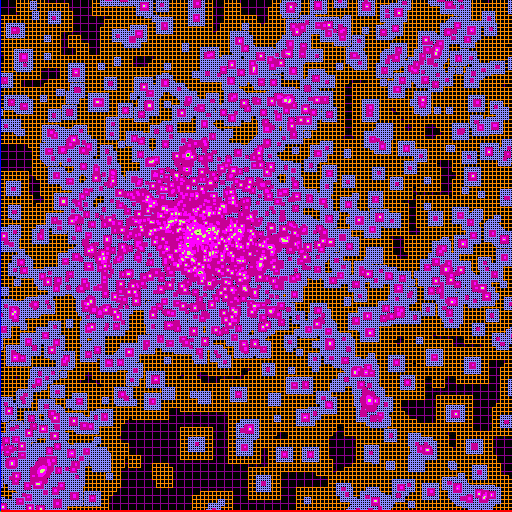
\includegraphics[width=\linewidth]{img/amr.png}
      \vskip 1cm
      {\huge \textbf{RAMSES~User's~Guide}}
      \vskip 2cm
      \Large
                  Self-gravitating~fluid~dynamics\\
      \vskip 5mm  with~Adaptive~Mesh~Refinement\\
      \vskip 5mm  using~massively~parallel~computers.
      \vskip 2cm

      \begin{tabular}{m{0.4\textwidth}m{0.4\textwidth}@{}}
      
\includegraphics[height=4cm]{img/irfu.pdf} & {\hfill \large Romain Teyssier} 
      \end{tabular}
   \end{minipage}
   \vfill
   \dblrule
   \flushright
   Version Issue: Version 3.0. Last Update: \today
\end{titlepage}

   % Table of contents
   \cleardoublepage
   \tableofcontents

   % Body
   \clearpage
\section{Introduction}

The RAMSES package is intended to be a versatile platform to develop
applications using Adaptive Mesh Refinement for computational
astrophysics. The current implementation allows solving the Euler
equations in presence of self-gravity and cooling, treated as additional
source terms in the momentum and energy equations. The RAMSES code can
be used on massively parallel architectures when properly linked to the
MPI library. It can also be used on single processor machines without
MPI. Output files are generated using native RAMSES Fortran unformatted
files. A suite of post-processing routines is delivered within the
present release, allowing the user to perform a simple analysis of the
generated output files.

\subsection{About This Guide}

The goal of this User's Guide is to provide a step-by-step tutorial in
using the RAMSES code. This guide will first describe a simple example of
its use. More complex set-up will be addressed at the end of the
document. Typical RAMSES users can be grouped into 3 categories:

\begin{itemize}
   \item Beginners: It is possible to execute RAMSES using only run
parameter files. The code is compiled once, and the user only modifies
the input file to perform various simulations. Cosmological simulations
can be performed quite efficiently in this way, using the initial
conditions generated by external packages such as \pkg{mpgrafic}.
   \item Intermediate users: For more complex applications, the user can
easily modify a small set of routines in order to specify specific
initial or boundary conditions. These routines are called ``patches''
and the code should be recompiled each time these routines are
modified.
   \item Advanced users: It is finally possible to modify the base
scheme, add new equations, or add new routines in order to modify the
default RAMSES application. This guide will not describe these advanced
features. In this case, a new documentation would be given separately.
\end{itemize}

\subsection{Getting RAMSES}

RAMSES software can be downloaded in the \emph{Codes} section from various web
sites, the most frequently updated ones being the Bitbucket repository 
\url{https://bitbucket.org/rteyssie/ramses} and
\url{http://www.ics.uzh.ch/~teyssier/ramses}.  It is freely distributed under the CeCILL
software license (see section \ref{sec:cecill} and
\url{http://www.cecill.info/}) according the French legal system \emph{for
non-commercial use only}. For commercial use of RAMSES, please contact the
author, but be prepared for a massive financial compensation !

\subsection{Main features}
RAMSES contains various algorithms designed for:

\begin{itemize}
   \item Cartesian AMR grids in 1D, 2D or 3D
   \item Solving the Poisson equation with a Multi-grid and a Conjugate
Gradient solver
   \item Using various Riemann solvers (Lax-Friedrich, HLLC, exact) for
adiabatic gas dynamics
   \item Computing collision-less particles (dark matter and stars)
dynamics using a PM code
   \item Computing the cooling and heating of a metal-rich plasma due to
atomic physics processes and an homogeneous UV background (Haardt and
Madau model).
   \item Implementing a model of star-formation based on a standard
Schmidt law with the traditional set of parameters.
   \item Implementing a model of supernovae-driven winds based on a
local Sedov blast wave solution.
\end{itemize}

All these features can be used and parameterized using the RAMSES
parameter file, based on the Fortran ``namelist'' format.

\subsection{Acknowledgements}

The development of the RAMSES code has been initiated and coordinated by
the author. The author would like to thank all collaborators who took an
active role in the development of this version. They are cited in
chronological order.

\begin{itemize}
   \item Matthias Gonzalez and Dominique Aubert (initial conditions)
   \item St\'ephane Colombi and St\'ephanie Courty (cooling and atomic
physics)
   \item Yann Rasera (star formation, post-processing)
   \item Yohan Dubois (supernovae feedback)
   \item Thomas Guillet (multigrid Poisson solver)
   \item S\'ebastien Fromang, Patrick Hennebelle and Emmanuel Dormy (MHD
solver).
   \item Philippe Wautelet and Philippe S\'eri\`es (code optimization)
\end{itemize}

I would like to thank my collaborators for helping me developing more
advanced versions of RAMSES, not yet available as complete releases,
since it is mostly work in progress.

\begin{itemize}
   \item Beno\^it Commer\c{c}on (thermal conduction)
   \item \'Edouard Audit and Dominique Aubert (radiative transfer)
   \item R\'emi Abgrall and Richard Saurel (multifluid)
\end{itemize}

\subsection{The CeCILL License}
\label{sec:cecill}

This software is under Copyright of CEA and its author, Romain Teyssier.

This software is governed by the CeCILL license under French law and
abiding by the rules of distribution of free software. You can use,
modify and/or redistribute the software under the terms of the CeCILL
license as circulated by CEA, CNRS and INRIA at the following URL:
\url{http://www.cecill.info/}.

As a counterpart to the access to the source code and rights to copy,
modify and redistribute granted by the license, users are provided only
with a limited warranty and the software's author, the holder of the
economic rights, and the successive licensors have only limited
liability.

In this respect, the user's attention is drawn to the risks associated
with loading, using, modifying and/or developing or reproducing the
software by the user in light of its specific status of free software,
that may mean that it is complicated to manipulate, and that also
therefore means that it is reserved for developers and experienced
professionals having in-depth IT knowledge. Users are therefore
encouraged to load and test the software's suitability as regards their
requirements in conditions enabling the security of their systems and/or
data to be ensured and, more generally, to use and operate it in the
same conditions as regards security.

The fact that you are presently reading this means that you have had
knowledge of the CeCILL license and that you accept its terms.


   \clearpage
\section{Getting started}

In this section, we will explain step by step how to get the RAMSES
package and install it, then how to perform a simple test to check the
installation.

\subsection{Obtaining the package}

The package can be downloaded from the web site
\url{http://www-dapnia.cea.fr/Projets/COAST} in the \emph{Codes}
section. You will get a tar ball named \cmd{ramses.tar.gz}. The first
thing to do is to un-tar the archive on your preferred computer's home
directory.

\begin{Prompt}
\$ gunzip ramses.tar.gz | tar xvf
\end{Prompt}

This will create a new directory named \dir{ramses/}. In this directory,
you will find the following directory list

%TODO Update dir list
\begin{Verbatim}
amr/  bin/  doc/  hydro/  mhd/  namelist/  patch/  pm/  poisson/  utils/
\end{Verbatim}

Each directory contains a set of files with a given common purpose. For
example, \dir{amr/} contains all F90 routines dealing with the AMR grid
management and MPI communications, while \dir{hydro/} obviously contains
all F90 routines dealing with hydrodynamics. The first directory you are
interested in is the \dir{bin/} directory, in which the code will be
compiled.

\subsection{Compiling the code}

In this \dir{bin/} directory, you will find a Makefile. The first thing
to do is to edit the Makefile and modify the two variables \cflag{F90}
and \cflag{FFLAGS}. Several examples corresponding to different Fortran
compilers are given. The default values are:

\begin{Prompt}
F90=pgf90
FFLAGS=-Mpreprocess -DWITHOUTMPI -DNDIM=$(NDIM) -DSOLVER=$(SOLVER)
\end{Prompt}

The first variable is obviously the command used to invoke the Fortran
compiler. In this case, this is the Portland Group compiler. The second
variable contains Fortran flags and preprocessor directives. The first
directive, \cmd{-D}\cflag{WITHOUTMPI}, when used, switches off all MPI
routines. On the other hand, if you don't use this directive, the code
must be linked to the MPI library. We will discuss this point later.
Theses directives are called \emph{Compilation Time Parameters}.  They
should be defined within the Makefile. Default values are:

\begin{Prompt}
NDIM=1
SOLVER=hydro
\end{Prompt}

The first variable, \cflag{NDIM}, sets the dimensionality of the
problem. The default value is for 1D, plan-parallel flows. Allowed
values are 1, 2 and 3. The second directive defines the solver, which in
the current release of RAMSES can be \solver{hydro} or \solver{mhd}.
Other solvers are currently under development, such as \solver{rad},
\solver{diff} and so on.

There are 3 other preprocessor directives that can be use in RAMSES:
\cmd{-D\cflag{NVAR}=\cflag{NDIM}+2}, useful to set more variables in the
hydro solver, \cmd{-D\cflag{NPRE}=8}, to set the number of bytes used
for real numbers. \cmd{\cflag{NPRE}=8} corresponds to double precision
arithmetic and \cmd{NPRE=4} to single precision. This option is useful
to save memory during memory intensive runs. Finally, you can use
\cmd{-D\cflag{NVECTOR}=500} to set the size of the vector sweeps for
computationally intensive operations.

To compile RAMSES, execute:

\begin{Prompt}
\$ make
\end{Prompt}

If everything goes well, all source files will be compiled and linked
into an executable called \cmd{ramses1d}.

\subsection{Executing the test case}

To test the compilation, you need to execute a simple test case. Go up
one level and type the following command:

\begin{Prompt}
\$ bin/ramses1d namelist/{\nmlfilename}
\end{Prompt}

The first part of the command is the executable, and the second part, the only
command line argument, is an input file containing all \emph{Run Time
Parameters}. Several examples of such parameter files are given in the
\dir{namelist/} directory. The run we have just performed, \cmd{\nmlfilename},
is the Sod's test, a simple shock tube simulation in 1D. For comparison, we now
show the last {\lastlinescount} lines of standard output:

% TODO : check machine prec here
% NPREC=8
\logfile[\lastlinesln]{autolog/lastlines.log}

To save the standard output in a file, the user is encouraged to
redirect the standard output in a \emph{Log File}, in which all
control variables are outputted and stored, as well as simulation data
for 1D cases only

% TODO: give a reference log in distribution? (make test)
\begin{Prompt}
\$ bin/ramses1d namelist/{\nmlfilename} > {\logfilename}
\end{Prompt}
%
To monitor the progress of longer runs, you can also redirect standard output
to both a log file and the terminal at the same time with:
%
\begin{Prompt}
\$ bin/ramses1d namelist/{\nmlfilename} | tee {\logfilename}
\end{Prompt}

\clearpage % long log file follows !
\subsection{Reading the Log File}
We will now briefly describe the structure and the nature of the
information available in the Log Files. We will use as example the file
\cmd{\logfilename}, which should contain, starting from the top

\logfile{autolog/logstart.log}
%
\hskip 2cm \vdots
%
\logfile[\finestepln]{autolog/finestep.log}

After the code banner and copyrights, the first line indicates that you are
currently using 1 processor and 1 space dimension for this run. The code then
reports that it is building the initial AMR grid. The next lines give the
current mesh structure.

The first level of refinement in RAMSES covers the whole computational domain
with 2, 4 or 8 cells in 1, 2 or 3 space dimensions. The grid is then further
refined up to \nmlentry{levelmin}, which is this case is defined in the
parameter file to be \cmd{levelmin={\nmllevelmin}}.  The grid is then further
refined up to \nmlentry{levelmax}, which is in this case
\cmd{levelmax={\nmllevelmax}}. Each line in the Log File indicates the number
of octs (or grids) at each level of refinement. The maximum number of grids in
each level $l$ is equal to $2^{l-1}$ in 1D, to $4^{l-1}$ in 2D and to $8^{l-1}$
in 3D. The numbers inside parentheses give the minimum, maximum and average
number of grids per processor. This is obviously only relevant to parallel
runs.

The code then indicates the time integration starts. After outputting
the initial conditions to screen, the first \emph{Control Line} appears,
starting with the words \cmd{Fine step=}. The Control Line gives
information on each \emph{Fine Step}, its current number, its current
time coordinate, its current time step. Variable \logentry{a} is for
cosmology runs only and gives the current expansion factor. The last
variable is the percentage of allocated memory currently used by RAMSES
to store each flow variable on the AMR grid and to store each
collision-less particle, if any.

In RAMSES, adaptive time stepping is implemented, which results in defining
\emph{Coarse Steps} and \emph{Fine Steps}. Coarse Steps correspond to the
coarse grid, which is defined by variable \cmd{levelmin}. Fine Steps correspond
to finer levels, for which the time step has been recursively subdivided by a
factor of 2. Fine levels are ``sub-cycled'' twice as more as their parent
coarse level. This explains why, at the end of the Log File, only
{\coarsestepcount} Coarse Steps are reported ({\coarsestepfirst} through
{\coarsesteplast}), for {\finestepcount} Fine Steps (numbered {\finestepfirst}
to {\finesteplast}).

When a Coarse Step is reached, the code writes in the Log File the
current mesh structure. A new Control Line then appears, starting with
the words \cmd{Main step=}. This Control Line gives information on each
Coarse Step, namely its current number, the current error in mass
conservation within the computational box \logentry{mcons}, the current
error in total energy conservation \logentry{econs}, the gravitational
potential energy and the fluid total energy (kinetic plus thermal).

This constitutes the basic information contained in the Log File. In 1D
simulations, output data are also written to standard output, and thus to the
Log File. For 2D and 3D, output data are stored into unformatted Fortran binary
files.  1D data are shown using 5 columns (level of refinement, position of the
cell, density, velocity and pressure) as in the following Sod's test example:

\logfile[\lastoutputln]{autolog/lastoutput.log}

You can cut and paste the {\lastoutputncells} lines into another file and use
your favorite data viewer like \cmd{xmgrace} or \cmd{gnuplot} to visualize the
results.  These should be compared to the plots shown on Figure
\ref{fig:sod1d}. If you have obtained comparable numerical values and levels of
refinements, your installation is likely to be valid. You are encouraged to
edit the parameter file \cmd{\logfilename} and play around with other parameter
values, in order to test the code performances. You can also use other
Parameter Files in the \dir{namelist/} directory.

\begin{figure}
   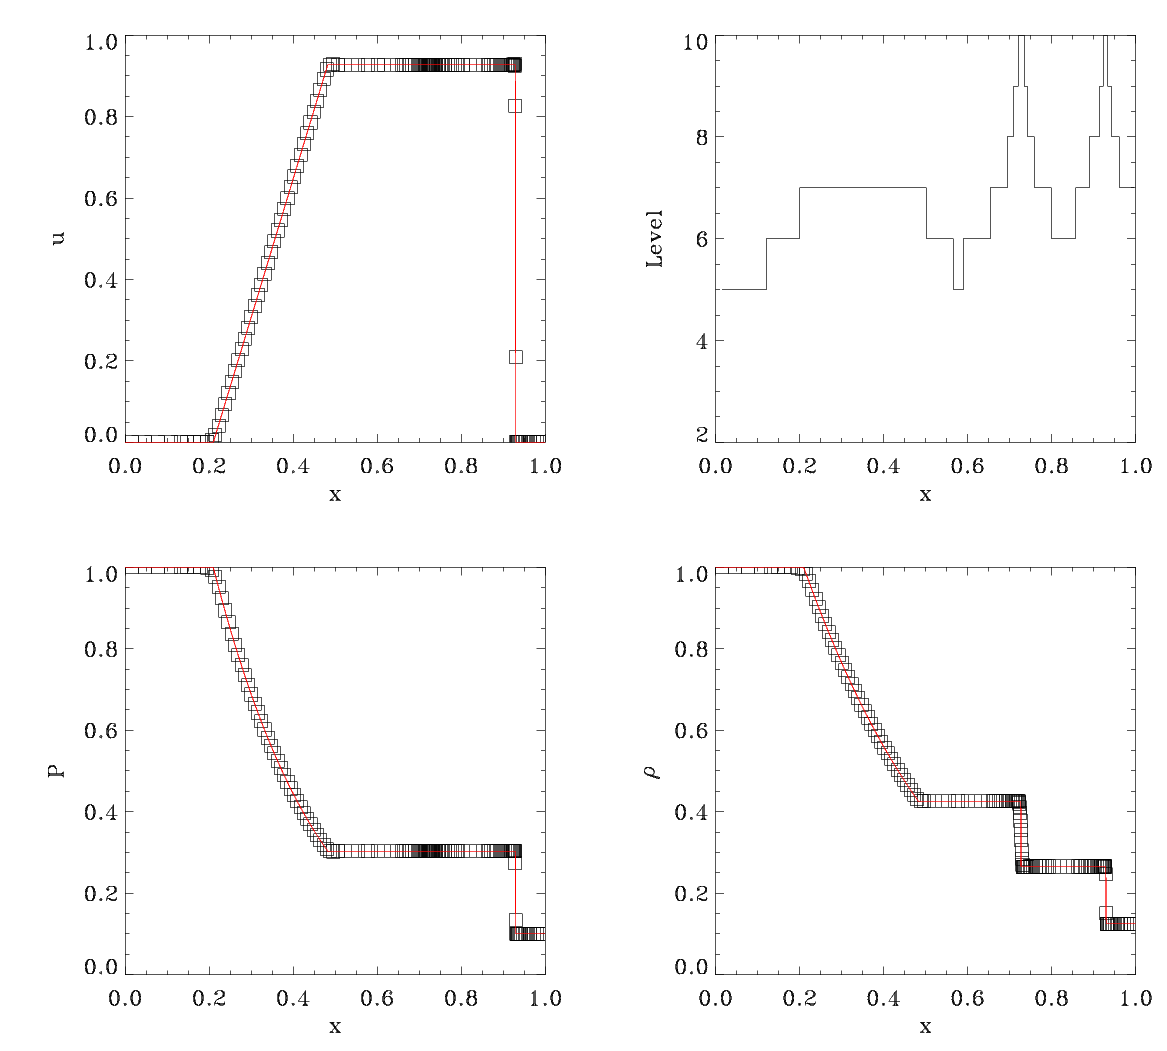
\includegraphics[width=\textwidth]{img/sod.png}
   \caption{Numerical results obtained with RAMSES for the Sod shock
tube test (symbols) compared to the analytical solution (red line).}
   \label{fig:sod1d}
\end{figure}


\begin{warning}
   Do not forget to recompile entirely the code (\cmd{make clean}, then
\cmd{make}) with \cflag{NDIM}\cmd{=2} for 2D cases like \cmd{sedov2d.nml} or
\cmd{NDIM=3} for 3D cases such as \cmd{sedov3d.nml}.
\end{warning}

In the next section, we will describe in more detail the various
Runtime Parameters available within RAMSES.


   \clearpage
\section{Runtime Parameters}

The RAMSES parameter file is based on the Fortran namelist syntax. The
Sod test parameter file is shown below, as it should appear if you edit
it.

\logfile{\fullnmlfilename}

This parameter file is organized in namelist blocks. Each block starts
with \cmd{\&BLOCK\_NAME} and ends with the character ``\cmd{/}''. Within
each block, you can specify parameter values using standard Fortran
namelist syntax. There are currently 9 different parameter blocks
implemented in RAMSES.

\begin{warning}
4 parameter blocks are mandatory and must always be present in the
parameter file. These are \nmlblock{\&RUN\_PARAMS},
\nmlblock{\&AMR\_PARAMS}, \nmlblock{\&OUTPUT\_PARAMS} and
\nmlblock{\&INIT\_PARAMS}.
\end{warning}

The 5 other blocks are optional. They must be present in the file only
if they are relevant to the current run. These are
\nmlblock{\&BOUNDARY\_PARAMS}, \nmlblock{\&HYDRO\_PARAMS},
\nmlblock{\&PHYSICS\_PARAMS}, \nmlblock{\&POISSON\_PARAMS} and finally
\nmlblock{\&REFINE\_PARAMS}. We now describe each parameter block in
more detail.

\clearpage
\subsection{Global parameters}

This block, called \nmlblock{\&RUN\_PARAMS}, contains the run global
control parameters. These parameters are now briefly described. More
thorough explanations will be given in dedicated sections.

\begin{nmltable}
   \cmd{\nmlentry{cosmo}=.false.} & Logical &
   Activate cosmological ``super-comoving coordinates'' system and
   expansion factor computing.
\\\midrule
   \cmd{\nmlentry{pic}=.false.} & Logical &
   Activate Particle-In-Cell solver
\\\midrule
   \cmd{\nmlentry{poisson}=.false.} & Logical &
   Activate Poisson solver.
\\\midrule
   \cmd{\nmlentry{hydro}=.false.} & Logical &
   Activate hydrodynamics or MHD solver.
\\\midrule
   \cmd{\nmlentry{verbose}=.false} & Logical &
   Activate verbose mode
\\\midrule
   \cmd{\nmlentry{nrestart}=0} & Integer &
   Output file number from which the code loads backup data and resumes
the simulation. The default value, zero, is for a fresh start from the
beginning. You should use the same number of processors than the one
used during the previous run.
\\\midrule
   \cmd{\nmlentry{nstepmax}=1000000} & Integer &
   Maximum number of coarse time steps.
\\\midrule
   \cmd{\nmlentry{ncontrol}=1} & Integer &
   Frequency of screen output for Control Lines (to standard output)
into the Log File).
\\\midrule
   \cmd{\nmlentry{nremap}=0} & Integer &
   Frequency of calls, in units of coarse time steps, for the load
balancing routine, for MPI runs only, the default value, zero, meaning
``never''. 
\\\midrule
   \cmd{\nmlentry{ordering}='hilbert'} & Character LEN=128 &
   Cell ordering method used in the domain decomposition of the grid
among the processors, for MPI runs only. Possible values are
\nmlentry{hilbert}, \nmlentry{planar} and \nmlentry{angular}.
   % TODO : BISECTION?
\\\midrule
   \cmd{\nmlentry{nsubcycle}=2,2,2,2,2,} & Integer array &
   Number of fine level sub-cycling steps within one coarse level time step.
Each value corresponds to a given level of refinement, starting from the coarse
grid defined by \nmlentry{levelmin}, up to the finest level defined by
\nmlentry{levelmax}. For example, \cmd{nsubcycle(1)=1} means that
\cmd{levelmin} and \cmd{levelmin+1} are synchronized.  To enforce single time
stepping for the whole AMR hierarchy, you need to set
\cmd{nsubcycle=1,1,1,1,1,}
\end{nmltable}


\clearpage
\subsection{AMR grid}

This set of parameters, called \nmlblock{\&AMR\_PARAMS}, controls the
AMR grid global properties. Parameters specifying the refinement
strategy are described in the \nmlblock{\&REFINE\_PARAMS} block, which is
used only if \nmlentry{levelmax}\cmd{>}\nmlentry{levelmin}.

\begin{nmltable}
   \cmd{\nmlentry{levelmin}=1} & Integer &
   Minimum level of refinement. This parameter sets the size of the
coarse (or base) grid by $n_x = 2^{\mathtt{levelmin}}$
\\\midrule
   \cmd{\nmlentry{levelmax}=1} & Integer &
   Maximum level of refinement. If \cmd{\mbox{levelmax}=levelmin}, this
corresponds to a standard cartesian grid.
\\\midrule
   \cmd{\nmlentry{ngridmax}=0} & Integer &
   Maximum number of grids (or octs) that can be allocated during the
run \emph{within each MPI process}.
\\\midrule
   \cmd{\nmlentry{ngridtot}=0} & Integer &
   Maximum number of grids (or octs) that can be allocated during the
run \emph{for all MPI processes}. One has in this case
\cmd{ngridmax=ngridtot/ncpu}.
\\\midrule
   \cmd{\nmlentry{npartmax}=0} & Integer &
   Maximum number of particles that can be allocated during the run
\emph{within each MPI process}.
\\\midrule
   \cmd{\nmlentry{nparttot}=0} & Integer &
   Maximum number of particles that can be allocated during the run
\emph{for all MPI processes}. Obviously, one has in this case
\cmd{\mbox{npartmax}=nparttot/ncpu}.
\\\midrule
   \cmd{\nmlentry{nexpand}=1} & Integer &
   Number of mesh expansions (mesh smoothing).
\\\midrule
   \cmd{\nmlentry{boxlen}=1.0} & Real &
   Box size in user units
\end{nmltable}


\clearpage
\subsection{Initial conditions}

This namelist block, called \nmlblock{\&INIT\_PARAMS}, is used to set up
the initial conditions.

\begin{nmltable}
   \cmd{\nmlentry{nregion}=1} & Integer &
   Number of independent regions in the computational box used to set up
   initial flow variables.
\\\midrule
   \cmd{\nmlentry{region\_type}='square'} & Character LEN=10 array &
   Geometry defining each region. \cmd{square} defines a generalized
ellipsoidal shape, while \cmd{point} defines a delta function in the
flow.
\\\midrule
   \nmlparbox{ \cmd{%
   \nmlentry{x\_center}=0.0\\
   \nmlentry{y\_center}=0.0\\
   \nmlentry{z\_center}=0.0}}
   &
   Real arrays
   &
   Coordinates of the center of each region.
\\\midrule
   \nmlparbox{\cmd{%
   \nmlentry{length\_x}=0.0\\
   \nmlentry{length\_y}=0.0\\
   \nmlentry{length\_z}=0.0}}
   &
   Real arrays
   &
   Size in all directions of each region.
\\\midrule
   \cmd{\nmlentry{exp\_region}=2.0}
   &
   Real array
   &
   Exponent defining the norm used to compute distances for the
generalized ellipsoid.
   \cmd{exp\_region=2} corresponds to a spheroid,
   \cmd{exp\_region=1} to a diamond shape, \cmd{exp\_region>=10} to a
perfect square.
\\\midrule
   \nmlparbox{\cmd{%
   \nmlentry{d\_region}=0.0\\
   \nmlentry{u\_region}=0.0\\
   \nmlentry{v\_region}=0.0\\
   \nmlentry{w\_region}=0.0\\
   \nmlentry{p\_region}=0.0}}
   &
   Real arrays
   &
   Flow variables in each region (density, velocities and pressure). For
\cmd{point} regions, these variables are used to defined extensive
quantities (mass, velocity and specific pressure).
\\\midrule
   \cmd{\nmlentry{filetype}='ascii'}
   &
   Character LEN=20
   &
   Type of initial conditions file for particles. Possible choices are
\cmd{'ascii'} or \cmd{'grafic'}.
\\\midrule
   \cmd{\nmlentry{aexp\_ini}=10.0}
   &
   Real
   &
   This parameter sets the starting expansion factor for cosmology runs
only. Default value is read in the IC file (\cmd{'grafic'} or
\cmd{'ascii'}).
\\\midrule
   \cmd{\nmlentry{multiple}=.false.}
   &
   Logical
   &
   If \cmd{.true.}, each processor reads its own IC file (\cmd{'grafic'}
or \cmd{'ascii'}). For parallel runs only.
\\\midrule
   \cmd{\nmlentry{initfile}=' '}
   &
   Character LEN=80 array
   &
   Directory where IC files are stored. See section \ref{sec:cosmo_init}
for details.
\end{nmltable}


\clearpage
\subsection{Output parameters}

This namelist block, called \nmlblock{\&OUTPUT\_PARAMS}, is used to set
up the frequency and properties of data output to disk.

\begin{nmltable}
   \cmd{\nmlentry{noutput}=1} & Integer &
   Number of specified output time. At least one output time should be
given, corresponding to the end of the simulation. 
\\\midrule
   \cmd{\nmlentry{tout}=0.0,0.0,0.0,} & Real array &
   Value of specified output time.
\\\midrule
   \cmd{\nmlentry{aout}=1.1,1.1,1.1,} & Real array &
   Value of specified output expansion factor (for cosmology runs only).
\cmd{aout=1.0} means ``present epoch'' or ``zero redshift''.
\\\midrule
   \cmd{\nmlentry{foutput}=1000000} & Integer &
   Frequency of additional outputs in units of coarse time steps.
\cmd{foutput=1} means one output at each time step. Specified outputs
(see above) will not be superceded by this parameter.
\end{nmltable}


\clearpage
\subsection{Boundary conditions}

This namelist block, called \nmlblock{\&BOUNDARY\_PARAMS}, is used to set up
boundary conditions on the current simulation. If this namelist block is
absent, periodic boundary conditions are assumed. Setting up other types of
boundary conditions in RAMSES is quite complex. The reader is invited to read
the corresponding section. The default setting, corresponding to a periodic box
should be sufficient in most cases. The strategy to set up boundary conditions
is based on using ``ghost regions'' outside the computational domain, where
flow variables are carefully specified in order to mimic the effect of the
chosen type of boundary. Note that \emph{the order in which boundary regions
are specified in the namelist is very important}, especially for reflexive or
zero gradient boundaries. See section \ref{sec:bc} for more information on
setting up such boundary conditions. Specific examples can be found in the
\dir{namelist/} directory of the package.

\begin{nmltable}
   \cmd{\nmlentry{nboundary}=1} & Integer &
   Number of ghost regions used to specify the boundary conditions. 
\\\midrule
   \cmd{\nmlentry{bound\_type}=0,0,0,} & Integer array &
   \nmlparbox{
   Type of boundary conditions to apply in the corresponding ghost region.
   Possible values are:\\
   \cmd{bound\_type=0}: periodic,\\
   \cmd{bound\_type=1}: reflexive,\\
   \cmd{bound\_type=2}: outflow (zero gradients),\\
   \cmd{bound\_type=3}: inflow (user specified).
   }
\\\midrule
   \nmlparbox{
      \cmd{\nmlentry{d\_bound}=0.0} \\
      \cmd{\nmlentry{u\_bound}=0.0} \\
      \cmd{\nmlentry{v\_bound}=0.0} \\
      \cmd{\nmlentry{w\_bound}=0.0} \\
      \cmd{\nmlentry{p\_bound}=0.0}
   }
   &
   Real arrays
   &
   Flow variables in each ghost region (density, velocities and
pressure).  They are used only for inflow boundary conditions. 
\\\midrule
   \nmlparbox{
      \cmd{\nmlentry{ibound\_min}=0} \\
      \cmd{\nmlentry{jbound\_min}=0} \\
      \cmd{\nmlentry{kbound\_min}=0}
   }
   &
   Integer arrays
   &
   Coordinates of the lower, left, bottom corner of each boundary
region.  Each coordinate lies between $-1$ and $+1$ in each direction (see
figure \vref{fig:bc}).
\\\midrule
   \nmlparbox{
      \cmd{\nmlentry{ibound\_max}=0} \\
      \cmd{\nmlentry{jbound\_max}=0} \\
      \cmd{\nmlentry{kbound\_max}=0}
   }
   &
   Integer arrays
   &
   Likewise, for the upper, right and upper corner of each boundary
region. 
\end{nmltable}


\clearpage
\subsection{Hydrodynamics solver}

This namelist is called \nmlblock{\&HYDRO\_PARAMS}, and is used to
specify runtime parameters for the Godunov solver. These parameters are
quite standard in computational fluid dynamics. We briefly describe them
now.

\begin{nmltable}
   \cmd{\nmlentry{gamma}=1.4} & Real &
   Adiabatic exponent for the perfect gas EOS. 
\\\midrule
   \cmd{\nmlentry{courant\_factor}=0.5} & Real &
   CFL number for time step control (less than 1).
\\\midrule
   \cmd{\nmlentry{smallr}=1d-10} & Real &
   Minimum density to prevent floating exceptions. 
\\\midrule
   \cmd{\nmlentry{smallc}=1d-10} & Real &
   Minimum sound speed to prevent floating exceptions. 
\\\midrule
   \cmd{\nmlentry{riemann}='llf'} & Character LEN=20 &
   Name of the desired Riemann solver. Possible choices are
   \cmd{'\rsolver{exact}'}, \cmd{'\rsolver{acoustic}'}, \cmd{'\rsolver{llf}'},
   \cmd{'\rsolver{hll}'} or \cmd{'\rsolver{hllc}'} for the hydro solver and
   \cmd{'\rsolver{llf}'}, \cmd{'\rsolver{hll}'}, \cmd{'\rsolver{roe}'},
   \cmd{'\rsolver{hlld}'}, \cmd{'\rsolver{upwind}'} and \cmd{'\rsolver{hydro}'}
   for the MHD solver.
\\\midrule
   \cmd{\nmlentry{riemann2d}='llf'} & Character LEN=20 &
   Name of the desired 2D Riemann solver for the induction equation (MHD
   only). Possible choices are \cmd{'upwind'}, \cmd{'llf'}, \cmd{'roe'}, \cmd{'hll'},
   and \cmd{'hlld'}.
\\\midrule
   \cmd{\nmlentry{niter\_riemann}=10} & Integer &
   Maximum number of iterations used in the exact Riemann solver.
\\\midrule
   \cmd{\nmlentry{slope\_type}=1} & Integer &
   \nmlparbox{
   Type of slope limiter used in the Godunov scheme for the piecewise
   linear reconstruction: \\
      \cmd{slope\_type=0}: First order scheme, \\
      \cmd{slope\_type=1}: MinMod limiter, \\
      \cmd{slope\_type=2}: MonCen limiter. \\
      \cmd{slope\_type=3}: Multi-dimensional MonCen limiter. \\
   In 1D runs only, it is also possible to choose: \\
      \cmd{slope\_type=4}: Superbee limiter \\
      \cmd{slope\_type=5}: Ultrabee limiter
   } 
\\\midrule
   \cmd{\nmlentry{pressure\_fix}=.false.} & Logical &
   Activate hybrid scheme (conservative or primitive) for high-Mach
   flows. Useful to prevent negative temperatures. 
\end{nmltable}


\clearpage
\subsection{Physical parameters}

This namelist, called \nmlblock{\&PHYSICS\_PARAMS}, is used to specify
physical quantities used in cosmological applications (cooling, star
formation and supernovae feedback). We briefly describe them now. 

\begin{nmltable}
   \cmd{\nmlentry{cooling}=.false.} & Logical &
   Activate the cooling and/or heating source term in the energy
equation.
\\\midrule
   \cmd{\nmlentry{metal}=.false.} & Logical &
   Activate metal enrichment, advection and cooling. \ In this case,
the preprocessor directive \mbox{\cmd{-D\cflag{NVAR}=6}} should be added in the
Makefile before the compilation. 
\\\midrule
   \cmd{\nmlentry{haardt\_madau}=.false.} & Logical &
   Use the UV background model of Haardt and Madau. Default value
\cmd{.false.} corresponds to a simple analytical model with parameters
\cmd{J21} and \cmd{a\_spec}. 
\\\midrule
   \cmd{\nmlentry{J21}=0.0} & Real &
   Normalization for the UV flux of the simple background model. Default
means ``no UV''. 
\\\midrule
   \cmd{\nmlentry{a\_spec}=1.0} & Real &
   Slope for the spectrum of the simple background model. Default value
corresponds to a standard ``quasars + OB stars'' spectrum.
\\\midrule
   \cmd{\nmlentry{z\_ave}=0.0} & Real &
   Average metallicity used in the cooling function, in case
\cmd{metal=.false.} 
\\\midrule
   \cmd{\nmlentry{t\_star}=0.0 } & Real &
   Star formation time scale in Gyr. Default value of zero means no star
formation. 
\\\midrule
   \cmd{\nmlentry{n\_star}=0.1, \nmlentry{del\_star}=200.0 }
   &
   Real
   &
   Typical interstellar medium physical density or comoving
overdensity, used as star formation density threshold and as EOS density
scale. 
\\\midrule
   \cmd{\nmlentry{T2\_star}=0.0, \nmlentry{g\_star}=1.6 }
   &
   Real
   &
   Typical interstellar medium polytropic EOS parameters.
\\\midrule
   \cmd{\nmlentry{eta\_sn}=0.0, \nmlentry{yield}=0.1 }
   &
   Real
   &
   Mass fraction of newly formed stars that explode into supernovae.
Default value of zero means no supernovae feedback.
\end{nmltable}


\clearpage
\subsection{Poisson solver}

This namelist, \nmlblock{\&POISSON\_PARAMS}, is used to specify runtime
parameters for the Poisson solver. It is used only if
\cmd{\nmlentry{poisson}=.true.} or \cmd{\nmlentry{pic}=.true.}

Two different Poisson solvers are available in RAMSES: conjugate gradient (CG)
and multigrid (MG). Unlike the CG solver, MG has an initialization overhead cost (at
every call of the solver), but is much more efficient on very big levels with
few ``holes''. The multigrid solver is therefore used for all coarse levels.

In addition, MG can be used on refined levels in conjuction with CG. The parameter
\nmlentry{cg\_levelmin} selects the Poisson solver as follows:
\begin{itemize}
\item Coarse levels are solved with MG
\item Refined levels with $l < \cmd{cg\_levelmin}$ are solved with MG
\item Refined levels with $l \geq \cmd{cg\_levelmin}$ are solved with CG
\end{itemize}

\begin{nmltable}
   \cmd{\nmlentry{gravity\_type}=0} & Integer &
   \nmlparbox{
      Type of gravity force. Possible choices are: \\
      \cmd{gravity\_type=0}: self-gravity (Poisson solver) \\
      \cmd{gravity\_type>0}: analytical gravity vector \\
      \cmd{gravity\_type<0}: self-gravity plus
      additional analytical density profile
   }
\\\midrule
   \cmd{\nmlentry{epsilon}=1d-4} & Real &
   Stopping criterion for the iterative Poisson solver: residual 2-norm
should be lower than \cmd{epsilon} times the right hand side 2-norm. 
   % TODO : update?
\\\midrule
   \cmd{\nmlentry{gravity\_params}=0.0, 0.0, 0.0, 0.0,}
   &
   Real array
   &
   Parameters used to define the analytical gravity field (routine
\cmd{gravana.f90}) or the analytical mass density field (routine
\cmd{rho\_ana.f90}).
\\\midrule
   \cmd{\nmlentry{cg\_levelmin}=999} & Integer &
   Minimum level from which the Conjugate Gradient solver is used in place
of the Multigrid solver.
\end{nmltable}


\clearpage
\subsection{Refinement strategy}

This namelist, \nmlblock{\&REFINE\_PARAMS}, is used to specify
refinement parameters controlling the AMR grid generation and evolution
during the course of the run. It is used only if
\nmlentry{levelmax} \cmd{>} \nmlentry{levelmin}.

\begin{nmltable}
   \cmd{\nmlentry{mass\_sph}=0.0} & Real &
   Quasi-Lagrangian strategy: \cmd{mass\_sph} is used to set a typical
mass scale. For cosmo runs, its value is set automatically.
\\\midrule
   \cmd{\nmlentry{m\_refine}=-1.,-1.,-1., } & Real array &
   Quasi-Lagrangian strategy: each level is refined if the baryons mass
in a cell exceeds \cmd{m\_refine(ilevel)*mass\_sph}, or if the number of
dark matter particles exceeds \cmd{m\_refine(ilevel)}, whatever the mass
is.
\\\midrule
   \cmd{\nmlentry{jeans\_refine}=-1.,-1.,} & Real array &
   Jeans refinement strategy: each level is refined if the cell size
exceeds the local Jeans length divided by \cmd{jeans\_refine(ilevel)}.
\\\midrule
   \nmlparbox{
      \cmd{\nmlentry{floor\_d}=1d-10},\\
      \cmd{\nmlentry{floor\_u}=1d-10},\\
      \cmd{\nmlentry{floor\_p}=1d-10}
   }
   &
   Real
   &
   Discontinuity-based strategy: density, velocity and pressure floor
below which gradients are ignored.
\\\midrule
   \nmlparbox{
      \cmd{\nmlentry{err\_grad\_d}=-1.0}, \\
      \cmd{\nmlentry{err\_grad\_u}=-1.0}, \\
      \cmd{\nmlentry{err\_grad\_p}=-1.0}
   }
   &
   Real
   &
   Discontinuity-based strategy: density, velocity and pressure relative
variations above which a cell is refined.
\\\midrule
   \nmlparbox{
      \cmd{\nmlentry{x\_refine}=0.0,0.0,0.0,}
      \cmd{\nmlentry{y\_refine}=0.0,0.0,0.0,}
      \cmd{\nmlentry{z\_refine}=0.0,0.0,0.0,}
   }
   &
   Real arrays
   &
   Geometry-based strategy: center of the refined region at each level
of the AMR grid. 
\\\midrule
   \nmlparbox{
      \cmd{\nmlentry{r\_refine}=1d10,1d10,} \\
      \cmd{\nmlentry{a\_refine}=1.0,1.0,} \\
      \cmd{\nmlentry{b\_refine}=1.0,1.0,} \\
      \cmd{\nmlentry{exp\_refine}=2.0,2.0,}
   }
   &
   Real arrays
   &
   Geometry-based strategy: size and shape of the refined region at each
level.
\\\midrule
   \cmd{\nmlentry{interpol\_var}=0}
   &
   Integer 
   &
   \nmlparbox{
      Variables used to perform interpolation (prolongation) and averaging
      (restriction). \\
      \cmd{interpol\_type=0}: conservatives ($\rho$, $\rho u$, $\rho E$) \\
      \cmd{interpol\_type=1}: primitives ($\rho$, $\rho u$, $\rho \epsilon$)
   }
\\\midrule
   \cmd{\nmlentry{interpol\_type}=1}
   &
   Integer 
   &
   \nmlparbox{
      Type of slope limiter used in the interpolation scheme for newly refined
      cells. \\
      \cmd{interpol\_type=0}: Straight injection (1\textsuperscript{st} order) \\
      \cmd{interpol\_type=1}: MinMod limiter, \\
      \cmd{interpol\_type=2}: MonCen limiter.
   }
\end{nmltable}



   \clearpage
\section{Cosmological simulations}

In this section, we describe in more detail how RAMSES can be used to
perform cosmological simulations. Useful concepts related to parallel
computing or post-processing will be introduced, and can also be used
for non-cosmological runs. Cosmological simulations are performed by
specifying \cmd{\nmlentry{cosmo}=.true.} in the \nmlblock{\&RUN\_PARAMS}
namelist.

\subsection{Parameter file and initial conditions}
\label{sec:cosmo_init}

The first thing to do when performing cosmological simulations is to
generate initial conditions as Gaussian random fields. The easiest way
is to use the freely available \pkg{grafic2} code, developed by Edmund
Bertschinger at MIT (see \url{http://web.mit.edu/edbert}) or its
parallel version \pkg{mpgrafic} developed by Christophe Pichon and Simon
Prunet at IAP (see \url{http://www.projet-horizon.fr/}). These codes
will generate initial conditions according to a given cosmological model
and for a given box size. As outputs, 7 files will be generated, called
\cmd{ic\_deltab}, \cmd{ic\_velcx}, \cmd{ic\_velcy}, \cmd{ic\_velcz},
\cmd{ic\_velbx}, \cmd{ic\_velby} and \cmd{ic\_velbz}. The directory in
which these files are stored should be entered in the Parameter File as
parameter \cmd{\nmlentry{initfile}(1)} in namelist
\nmlblock{\&INIT\_PARAMS}. Index 1 stands here for \nmlentry{levelmin},
and corresponds to the coarse grid.  RAMSES will automatically read the
cosmological parameters and the physical box length contained in these
initial conditions files. The so-called ``super-comoving'' coordinate
system is used in RAMSES for cosmological runs (see Martell \& Shapiro
2003). \ If necessary, the translation from this scale-free coordinate
system (\cmd{\nmlentry{boxlen}=1.0}) to the \emph{cgs} system is
performed using scaling factors stored in the output files. The units
are set in routine \cmd{units.f90} in directory \dir{amr/}.

The following namelist can be found in directory \dir{namelist/} in the
RAMSES package as file \cmd{cosmo.nml}. It is the Parameter File for a
pure $N$-body simulation, using $128^3$ particles and a $128^3$ coarse
grid with 7 additional levels of refinement. To specify that initial
conditions are to be read in grafic files,
\cmd{\nmlentry{filetype}='grafic'} should be set in namelist
\nmlblock{\&INIT\_PARAMS}. 

\logfile{userfiles/cosmo.nml}

Parameters \nmlentry{ngridtot} and \nmlentry{nparttot} specify the
maximum memory allocated for AMR grids and collisionless particles
respectively. These numbers should be greater than or equal to the
actual number of AMR grids and particles used during the course of the
simulation. 

\nmlentry{ngridtot} stands for the total number of AMR grids allocated
over all MPI processes. The \nmlentry{ngridmax} parameter can be used
equivalently, but stands for the local number of AMR grids within each
MPI process. Obviously, one has \cmd{ngridtot=ngridmax*ncpu}.

\begin{warning}
Recall that, in RAMSES, we call ``AMR grid'' or ``oct'' a group of
$2^{\mathtt{ndim}}$ cells. If for some reason, during the course of the
execution, the maximum allowed number of grids or particles has been
reached, the simulation stops with the message:
%
\begin{Prompt}
 No more free memory
 Increase ngridmax
\end{Prompt}
%
In this case, don't panic: just increase \nmlentry{ngridmax} in the
Parameter File and resume the execution, starting from the last backup
file. 
\end{warning}


\subsection{Memory management}

These two parameters control the memory allocated by RAMSES. It is
important to know how much memory in Gb is actually allocated by RAMSES
for a given choice of parameters. This can be approximated by:

\begin{itemize}
\item $0.7 (\nmlentry{ngridmax}/10^6) + 0.7 (\nmlentry{npartmax}/10^7)$
Gbytes for pure $N$-body runs,
\item $1.4 (\nmlentry{ngridmax}/10^6) + 0.7 (\nmlentry{npartmax}/10^7)$
Gb for $N$-body and hydro runs,
\item $1.0 (\nmlentry{ngridmax}/10^6)$ Gb for pure hydro runs. 
\end{itemize}

Because of MPI communications overheads, the actual memory used can be
slightly higher. Note that these numbers are valid for double precision
arithmetic. For single precision runs, using the preprocessor directive
\cmd{-D\cflag{NPRE}=4}, you can decrease these figures by 40\%. 
% TODO: warning about single precision here

\subsection{Restarting a run}

As we just discussed, it is possible to resume a RAMSES run if the
execution has stopped abnormally. For that, RAMSES uses its output
files, stored in directories called

\begin{Verbatim}
output_00001/
output_00002/
output_00003/
output_00004/
\end{Verbatim}

Each directory contains all the necessary information for RAMSES to
resume the execution. The frequency at which these output files are
created is specified by parameter \nmlentry{foutput}, in units of coarse
time steps. If you want to resume the execution starting from output
directory number 4, you need to specify the corresponding number in
parameter \cmd{\nmlentry{nrestart}=4}. If you set
\cmd{\nmlentry{nrestart}=0}, the run will start from the beginning as a
completely new run. 

\begin{warning}
When restarting a job, you can change almost all run parameters. There
are however some notable exceptions: The number of output times can only
be increased, and only new output times can be added after the old ones.
The number of processors used with MPI cannot change. If you want to
change the number of processes, you should start from the very
beginning.
\end{warning}

\subsection{Parallel computing}

We are now ready to address the complex issue of parallel computing
with RAMSES. It is based on the MPI library through regular calls of MPI
communication routines. In order to compile and link RAMSES with the MPI
library, you need first to remove the preprocessor directive
\cmd{-D\cflag{WITHOUTMPI}} from the compilation options in the Makefile.
Don't forget to type \cmd{make clean} and then \cmd{make} again.

In order to launch a parallel RAMSES run, type for example

\begin{Prompt}
\$ mpirun -np 4 bin/ramses3d namelist/sedov3d.nml 
\end{Prompt}

The two key parameters for parallel runs are \nmlentry{nremap} and
\nmlentry{ordering}, both contained in the \nmlblock{\&RUN\_PARAMS}
namelist block. The first one specifies the frequency at which the code
will optimize load balancing by adjusting the domain decomposition, in
units of coarse time step. Since it is a rather costly operation, this
should not be performed too frequently. On the other hand, if the AMR
grid evolves significantly with time, the computational and memory load
might be very inhomogeneous across the processors. The optimal choice
for parameter \nmlentry{nremap} is therefore application-dependent. Bear
in mind that if \cmd{nremap>10}, the associated overhead should be
negligible. 

The other important parameter for an efficient parallel computing
strategy is \nmlentry{ordering}. This character string specifies the type
of domain decomposition you want to use. There are 3 possible choices in
RAMSES currently implemented: \cmd{'hilbert'} (default value),
\cmd{'planar'} and \cmd{'angular'}. Each cell in RAMSES is ordered with
an integer index according to a given space ordering. One of the most
famous ordering used in computer science is the Peano-Hilbert
space-filling curve. This is a one-dimensional object filling up the
three-dimensional space. An example of such domain decomposition is
shown in figure \ref{fig:hilbert}. This strategy is known to be the
optimal choice if one considers the rather large ensemble of all
possible AMR grids. In some cases, however, it is no longer an
efficient strategy. The planar decomposition, for example, sets up
computational domains according to one coordinate only (the altitude $z$
for example). Each processor receives a layer of cells whose thickness
is automatically adjusted in order to optimize load balance. The angular
decomposition follows the same strategy, except that now the coordinate
is the polar angle around a given axis in the simulation box. These
various orderings can be adapted easily to account for specific
constraints. The user is encouraged to edit and modify the routine
\cmd{load\_balance.f90} in directory \dir{amr/}.

\begin{figure}
   \begin{center}
   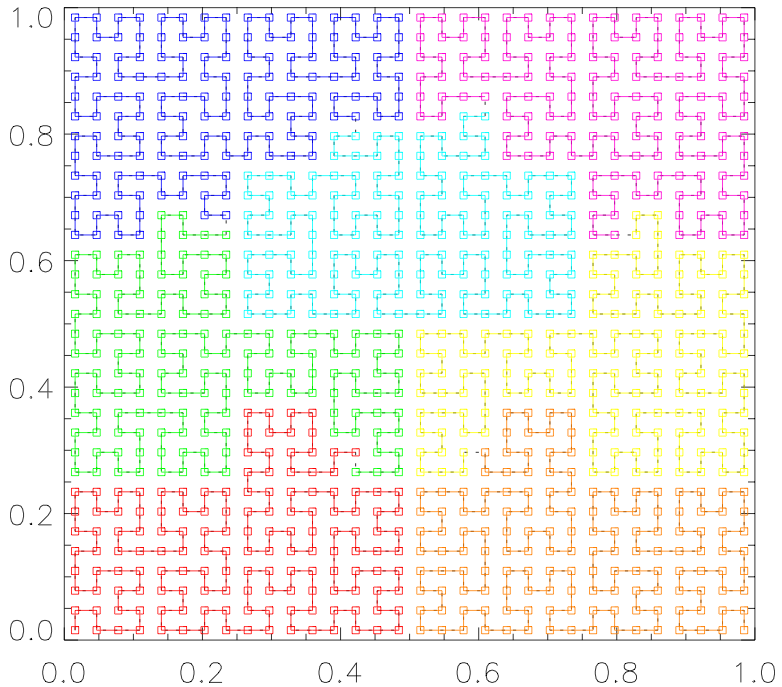
\includegraphics[width=0.8\textwidth]{img/hilbert.png}
   \end{center}
   \caption{Domain decomposition of the unit square for a $32^2$ grid
   over 7 processors using the Peano-Hilbert space-filling curve
   shown as the continuous line.}
   \label{fig:hilbert}
\end{figure}


In case of parallel execution, RAMSES performs hard disk outputs in a very
simple way: each processor creates its own file. Therefore, in directory
\dir{output\_00001/}, one can find several files with a numbering
corresponding to the processor number. One should bear this in mind when
using the snapshots generated by RAMSES.

\subsection{Post-processing utilities}

Several post-processing codes are available in the current package in
directory \dir{utils/f90}. These are very simple pieces of software
performing rather basic operations on RAMSES generated outputs. Users are
encouraged to edit and modify these routines in order to design specific
post-processing applications. We briefly describe them now.

\begin{itemize}
\item \util{amr2map}: this application reads RAMSES outputs and
generates a projected map along one principal axis. The output is a
binary Fortran image that can be read using any image-processing tool.
\item \util{amr2cube}: this application reads RAMSES outputs and
generates a 3D Cartesian cube with only one flow variable represented.
The output is a binary Fortran file (raw data or grafic data) or a VTK
file that can be read using any data visualization tool.
\item \util{part2map}: this application reads RAMSES outputs for
collisionless particles only and projected the particle distribution
along one principal axis. The output is a binary Fortran image.
\item \util{part2cube}: this application reads RAMSES outputs for
particles only and generates a CIC interpolated density field. The
output is a binary Fortran file.
\end{itemize}

Each one of these codes is a stand-alone application that can be
compiled straightforwardly by typing directly for example:

\begin{Prompt}
\$ f90 amr2map.f90 -o amr2map  
\end{Prompt}

In directory \dir{utils/idl}, you can find a set of IDL routines to be
used in order to display AMR data using IDL (see
\url{http://www.ittvis.com/}).  Here is an example of interactive
commands you need to type within your IDL session to watch RAMSES data
(for example using \cmd{sedov2d.nml}). 

\begin{Prompt}
IDL> rd_amr,a,nout=2   ; Read AMR data from snapshot nr 2 and store in a
IDL> rd_hydro,h,nout=2 ; Read hydro data and store in variable h
IDL> window,0,xs=512,ys=512       ; Set up a square window
IDL> loadct,33                    ; Load a nice color table
IDL> tv2d,a,h,type=1,/log,/show   ; Plot a density map with the grid
\end{Prompt}
%
Here is another example to plot a density profile from the previous
data.
%
\begin{Prompt}
IDL> amr2cell,a,h,c        ; Convert AMR data into cell-based data
IDL> r=sqrt(c.x^2+c.y^2)   ; Compute cell radius
IDL> d=c.var(*,0)          ; Compute cell density
IDL> plot,r,d,psym=6
\end{Prompt}
%
For 3D data, you can use a simple raytracing algorithm to project
various quantities along one of the box principal axis.
%
\begin{Prompt}
IDL> ray3d,a,h,lmin=7,lmax=9,/zproj,/ave,type=1,/log
          ; Project the average density along the z-axis
\end{Prompt}


\subsection{Zoom simulations}

Another interesting cosmological application for RAMSES is the so-called
``zoom'' technology or ``re-simulation'' process. Let us consider the
large-scale periodic box simulation we have presented in the previous
section, performed with $128^3$ particles by RAMSES with the
\pkg{grafic} files stored in directory \cmd{/scratchdir/grafic\_files}.
After using the \util{sod} application, all dark matter halos in the
final output have been identified. One halo is believed to be a good
candidate for re-simulation. A quasi-spherical region must be
determined, whose size and position are optimized in order to contain
all the particles ending up in the final halo. A new set of initial
conditions must then be generated using \pkg{mpgrafic}, providing the
same large-scale modes than the previous run, but allowing now to
simulate up to $1024^3$ particles.
A suite of applications is available in directory \dir{utils/f90} to
perform the extraction of a high-resolution region containing the halo
particles only. These codes are called \util{center\_grafic},
\util{extract\_grafic} and \util{degrade\_grafic}. The idea is to center
the simulation box on the high-resolution region, to extract a nested
collection of rectangular grids around this position with various
particle masses.  The initial conditions data for each box are stored in
a different directory. The original data centered on the region center
can be called \cmd{boxlen100\_n256}, where \cmd{100} stands for the box
size in $h^{-1}$ Mpc and \cmd{128} for the number of particles per box
length. The nested box hierarchy we obtained using our various utilities
is now:
%
\begin{Verbatim}
boxlen100_n128/
boxlen50_n128/
boxlen25_n128/
boxlen12p5_n128/
\end{Verbatim}
%
Each of these directories should contain 7 grafic files. These names
should be now inserted in the Parameter File, in the
\nmlblock{\&INIT\_PARAMS} block, as
%
\begin{Verbatim}
&INIT_PARAMS
filetype='grafic'
initfile(1)='/scratchdir/grafic_directories/boxlen100_n128'
initfile(2)='/scratchdir/grafic_directories/boxlen50_n128'
initfile(3)='/scratchdir/grafic_directories/boxlen25_n128'
initfile(4)='/scratchdir/grafic_directories/boxlen12p5_n128'
/
\end{Verbatim}
%
The re-simulation is now ready to go. Those are our last words on
cosmological simulations and how to run them using only Parameter Files
as Runtime Parameters. We now describe how to use RAMSES with more
advanced settings.


   \clearpage
\section{Advanced simulations}

For truly innovative scientific applications, the user is usually forced to
define complex initial conditions, to impose time varying boundary conditions
or to use more than the 5 standard Euler variables (chemical species for
example).  We briefly describe the easiest way to do it in RAMSES.

\subsection{Patching the code}

The general philosophy to design advanced RAMSES applications is to ``patch the
code''. What do we mean by that? A few key routines have been designed in
RAMSES in a user-friendly fashion, allowing the user to edit the file,
modify it according to it needs and recompile the code. For that, it is
recommended to create your own directory, for example \cmd{mypatch/}, in which
you will copy the various files you plan to modify. In the \cmd{Makefile}, you
need to specify the complete path of this directory in the \cflag{PATCH}
variable, as:
%
\begin{Prompt}
PATCH=/home/foo/mypatch  
\end{Prompt}
%
The \cmd{make} command will seek for sources files in this directory first,
compile and link them if present. If not, it will use the default source
files already available in the RAMSES package. Virtually any RAMSES source file
can be modified to obtain a ``patched'' version of RAMSES that fulfill your
needs. Usually, however, only a few routines need to be modified in order to
perform advanced simulations.  These routines will be described now in more
detail. The corresponding files are stored in various RAMSES subdirectories.
These are: \cmd{amr/units.f90}, \cmd{hydro/boundana.f90},
\cmd{hydro/condinit.f90}, \cmd{poisson/gravana.f90},
\cmd{poisson/rho\_ana.f90}, \cmd{hydro/cooling\_fine.f90}. Of course, other
routines of RAMSES can be modified at will, although potential changes might be
more complicated to implement. A simple example of patch can be found in the
directory \dir{patch/} of the package. 

\subsection{Physical units}

This very simple routine can be found in directory \dir{amr/} and is called
\cmd{units.f90}. It is used to set the conversion factors from the user units
into the cgs unit system. In this routine, the user must provide 3 scaling
factors, namely \cmd{scale\_d} for the density units in
$\mathrm{g}.\mathrm{cm}^{-3}$, \cmd{scale\_l} for the length scale in cm and
\cmd{scale\_t} for the time scale in seconds. For self-gravity runs, since
RAMSES assumes $G=1$ in the Poisson equation, it is mandatory to define the
time scale as \cmd{scale\_t=1.0/sqrt(G*scale\_d)} with \cmd{G=6.67d-8}. These
scaling factors are stored in the output files and can be used later on during
post-processing.

\subsection{Initial conditions}

This routine can be found in directory \dir{hydro/} and is called
\cmd{condinit.f90}. It is self-documented. The calling sequence is just
\cmd{call condinit(x,u,dx,ncell}), where \cmd{x} is an input array of cell
center positions, \cmd{u} is an output array containing the volume average of
the fluid conservative variables, namely ($\rho$, $\rho u$, $\rho v$, $\rho w$
and $E$), in this exact order. If more variables are defined, using the
\cmd{-D\cflag{NVAR}} directive, then the user should exploit this routine to
define them too. \cmd{dx} is a single real value containing the cell size for
all the cells and \cmd{ncell} is the number of cells.  This routine can be used
to set the initial conditions directly with Fortran instructions. Examples of
such instructions can be found in directory \dir{patch/}.

Another way to define initial conditions in RAMSES is by using input files. For
the hydro solver, these files are always in the \pkg{grafic} format. We have
already explained how to use the \pkg{grafic} format for cosmological runs. For
non-cosmological runs, initial conditions can be defined using the exact same
format, except that instead of 4 files (\cmd{ic\_deltab}, \cmd{ic\_velbx},
\cmd{ic\_velby} and \cmd{ic\_velbz}), one now needs 5 files called
(\cmd{ic\_d}, \cmd{ic\_u}, \cmd{ic\_v}, \cmd{ic\_w} and \cmd{ic\_p}) and
containing the fluid primitive variables.

For collisionless particles, the \pkg{grafic} format is used only for
cosmological runs, for which particles are initially placed at the cell centers
of a Cartesian grid. For non-cosmological runs, the particles' initial
positions, velocities and masses are read in an ASCII file, in which each line
corresponds to one particle, and should contain the following particle
attributes: \cmd{x,y,z,vx,vy,vz,m}.

\subsection{Boundary conditions}
\label{sec:bc}

As explained in the previous sections, RAMSES can provide boundary conditions
of different types: periodic (default mode), reflexive, outflow and imposed.
This is performed in RAMSES using ghost regions, in which the fluid variables
are set in order to obtain the required boundary. Ghost regions are defined in
the namelist block \nmlblock{\&BOUNDARY\_PARAMS}. Each region is identified by
its position, its type and eventually by the value of the fluid variables. 

\begin{warning}
The exact order with which boundary regions are entered in the namelist block
is very important. Let us consider the 4 boundary regions shown in figure
\ref{fig:bc}. They are defined by the following namelist block:
%
\begin{Prompt}
&BOUNDARY_PARAMS
nboundary=4
ibound_min=-1,+1,-1,-1
ibound_max=-1,+1,+1,+1
jbound_min= 0, 0,+1,-1
jbound_max= 0, 0,+1,-1
bound_type= 1, 1, 1, 1
/
\end{Prompt}
%
The first region is located in the rectangle defined by coordinate
$(i=-1,j=0)$, while the third region is defined by coordinates $(-1 \leq i \leq
+1, j=+1)$. The boundary type for all 4 regions is set to ``reflexive''
(\cmd{\nmlentry{bound\_type}=1}). The fluid variables within the ghost region
are therefore taken equal to the values of their symmetric cells, with respect
to the boundary. This is why the order of the ghost regions is so important:
regions 1 and 2 are updated first, using only the fluid variables within the
computational domain.  Regions 3 and 4 are updated afterwards, using the fluid
variables within the computational domain, but also within regions 1 and 2. In
this way, all cells within boundary regions are properly defined, especially in
the 4 corners of the computational domain.
\end{warning}

It is possible to define only 2 regions (say regions 1 and 2 in figure
\ref{fig:bc}), the orthogonal direction will be considered as periodic. For
gravity runs, the gravitational force is also updated in the ghost regions,
following the same rules as the velocity vector.

\begin{figure}
   \begin{center}
   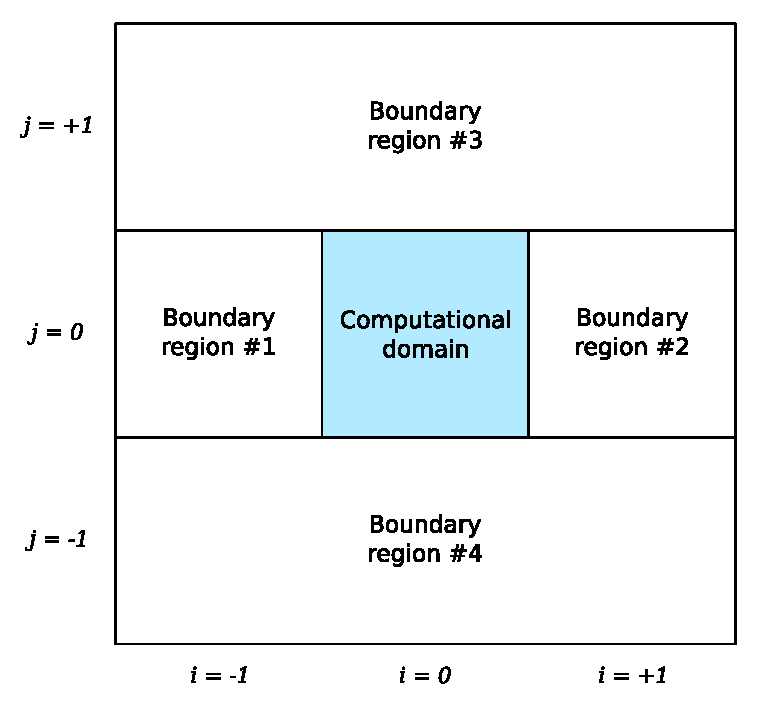
\includegraphics[width=0.65\textwidth]{img/bc.pdf}
   \end{center}
   \caption{Example of ghost regions used in RAMSES to impose specific boundary
conditions.}
   \label{fig:bc}
\end{figure}

For the Poisson equation, however, boundary conditions are either periodic, if
no ghost regions are defined in the corresponding direction, or ``$\phi=0$''
Dirichlet boundary conditions within ghost regions. No other types of boundary
conditions for the Poisson equation have been implemented (such as isolated,
reflexive and so on). 
% TODO update?

If \cmd{\nmlentry{bound\_type}=3}, boundary conditions must be imposed by the
user. The first possibility is to use parameters \nmlentry{d\_bound},
\nmlentry{u\_bound}{\dots} to set a constant fluid state within the desired
ghost region. For more advanced applications, the user is encouraged to patch
the routine \cmd{boundana.f90} within directory \cmd{hydro/}. This routine is
very similar to routine \cmd{condinit.f90}. The calling sequence is \cmd{call
boundana(x,u,dx,ibound,ncell}). The ghost region number is therefore provided,
so the user can specify some region-dependent fluid conditions.

\subsection{External gravity sources}

If \cmd{\nmlentry{bound\_type}=3}, boundary conditions must be imposed also for
the gravitational force. This is performed by modifying routine
\cmd{gravana.f90} in directory \dir{poisson/}. If \cmd{gravity\_type>0}, this
routine is also used to specify the gravitational force within the
computational domain. Note that in this case, the fluid is not self-gravitating
anymore. There is another way to impose an external gravity source and in the
same time, to solve for the Poisson equation. This is done using routine
\cmd{rho\_ana.f90} in directory \dir{poisson/}. In this routine, again very
similar to the previously presented Fortran routines, the user can specify the
density profile for the external gravity source.  This density profile will be
added to the fluid density as the source term in the Poisson equation.

\subsection{External thermal sources}

The final routine that can be easily modified by the user is
\cmd{cooling\_fine.f90} in directory \dir{hydro/}. This routine is used if
\cmd{\nmlentry{cooling}=.true.} or if the polytropic temperature
\cmd{\nmlentry{T2\_star}>0.0}. In the first case, cooling and heating source
terms are added to the energy equation and solved by a fully implicit
integration scheme. In the second case, the thermal energy of the fluid is not
allowed to be lower than a polytropic Equation-Of-State, for which one has $ T
/ \mu = {(T / \mu)}_{*} {(\rho / \rho_{*})}^{\gamma_{*}-1} $.  All starred
parameters can be set within the namelist block \nmlblock{\&PHYSICS\_PARAMS}.
On the other hand, the user might want to modify routine
\cmd{cooling\_fine.f90} in order to implement more complex thermal modeling of
the fluid.


   \clearpage
\section{Publication policy}

The RAMSES code is freely available for non-commercial use under the
CeCILL License agreement. If a paper is published with simulations
performed with RAMSES, the authors should cite the following paper, in
which the RAMSES code was presented for the first time:

% TODO : Better citing 
{ \itshape
Teyssier, Romain, ``Cosmological hydrodynamics with Adaptive Mesh
Refinement: a new high-resolution code called RAMSES'', Astronomy and
Astrophysics, 2002, volume 385, page 337 }

If the same users need some basic help from the author on how to use
RAMSES, or if the simulations performed have needed from the code's
author some small adaptation of the code, a small sentence like ``We
thank Romain Teyssier for{\dots}'' in the Acknowledgment section will do
it.

If, on the other hand, the simulations performed requires the code's
author to be more deeply involved in the project (new developments, new
simulations from the author's side), then co-authorship of the paper is
asked.


   % Index
   \clearpage
   \phantomsection
   \addcontentsline{toc}{section}{Index}
   \printindex

\end{document}
